\documentclass{article}
\usepackage[T1]{fontenc}
% DOC PRE-AMBLE
\usepackage[a4paper,margin={1in,1in}]{geometry}
\usepackage{hyperref}
\usepackage{graphicx}
\title{MPHYG001 Assignment 2: Refactoring Boids}
\author{\\
Danial Dervovic\\
\normalsize University College London\\
\normalsize \href{mailto:danial.dervovic.11@ucl.ac.uk}{\texttt{danial.dervovic.11@ucl.ac.uk}}
}
% CODE PRE-AMBLE
\usepackage{listings}
\lstset{language=bash, basicstyle=\ttfamily\footnotesize, keepspaces=true
showspaces=false,breaklines=true, showstringspaces=false, frame=single,
upquote=true}


\begin{document}
\maketitle
\section*{Introduction/Usage}
For this assignment, the task was to take the Boids code\footnote{\href{http://development.rc.ucl.ac.uk/training/engineering/ch05construction/10boids.html}{\texttt{http://development.rc.ucl.ac.uk/training/engineering/ch05construction/10boids.html}}}, packaging it up into a form that can be \texttt{pip} installed and run from the command line. This code may be found at the GitHub repository \href{https://github.com/ddervs/bad-boids}{\texttt{ddervs/bad-boids}}. The usage of the packaged function is shown below (the output of \texttt{boids -{}-help}).
\begin{lstlisting}
usage: boids [-h] [--config CONFIG] [--example_config]

Runs the boids simulation.

optional arguments:
  -h, --help        show this help message and exit
  --config CONFIG   YAML file with simulation options. See README.md or use
                    --example-config option for specification.
  --example_config  Saves default config file to current working directory.
\end{lstlisting}
\section*{Refactorings}
In this task, the refactoring approach was used. The common refactorings utilised are shown in Table~\ref{tab:refactor}.
\begin{center}[h]
\begin{tabular}{|c|c|}
    \hline
    \textbf{Code Smell} & \textbf{Commit number} \\
    \hline\hline
    Repeated Loops & \texttt{515da7c} \\
    Magic Numbers & \texttt{87c90c7} \\
    Turn \texttt{boids} into a class & \texttt{2ff425b} \\
    Repeated code/copypasta & \texttt{0128753} \\
    Many constants $\rightarrow$ config file & \texttt{a23e2fa} \\
    Large function into units & \texttt{fa117b3} \\
    Too many loops $\rightarrow$ \texttt{numpy} & \texttt{980ce16} \\
    \hline
\end{tabular}
The main advantage of such an approach is that at each stage, the code set still works as originally. 
\caption{Table of refactorings along with corresponding commit numbers.}
\label{tab:refactor}
\end{center}
\section*{UML Diagram}
\begin{figure}[h]
\centering
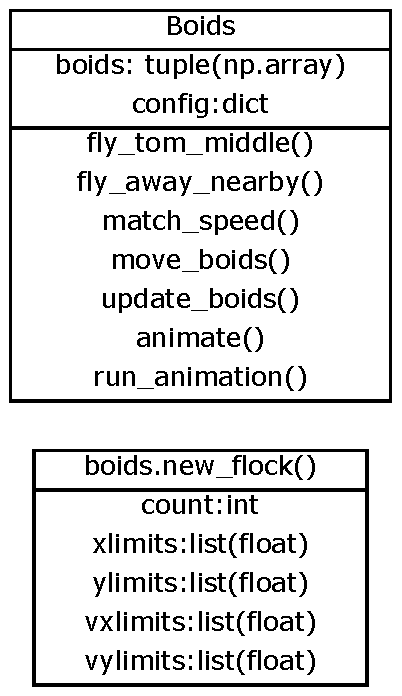
\includegraphics[width=0.25\textwidth]{UML}
\caption{UML diagram of \texttt{boids} package.}
\label{fig:UML}
\end{figure}

\end{document}
